\documentclass[11pt, a4paper, oneside]{ctexbook}
\usepackage{amsmath, amsthm, amssymb, bm, graphicx, hyperref, mathrsfs, enumitem, geometry, listings, xcolor, float, footmisc}
\title{{\Huge{\textbf{《中南大学\ 软件测试工程》}}}\\课后作业二}
\author{徐鸣飞}
\date{2023 年 10 月 27 日}
\linespread{1.5}

\newtheorem{theorem}{定理}[section]
\newtheorem{definition}[theorem]{定义}
\newtheorem{lemma}[theorem]{引理}
\newtheorem{corollary}[theorem]{推论}
\newtheorem{example}[theorem]{例}
\newtheorem{proposition}[theorem]{命题}

\geometry{a4paper,scale=0.8}


\begin{document}

\maketitle
\pagenumbering{roman}
\setcounter{page}{1}
\newpage
\pagenumbering{Roman}
\setcounter{page}{1}
\tableofcontents
\newpage
\setcounter{page}{1}
\pagenumbering{arabic}

\chapter{AI主播定义}
\section{定义}
AI主播是利用人工智能技术开发的虚拟主播,其主要功能是利用语音合成、自然语言处理和人脸识别等技术,以类似真人的方式进行信息传递、新闻播报、节目主持等活动。AI主播能够模拟人类的语音、语调、表情和动作,以及实时互动能力,使其看起来更加真实且具有吸引力。

AI主播在新闻媒体、电视台、网络直播平台和其他媒体渠道中得到了广泛应用。其优势包括可以24小时不间断地工作,不会出现疲劳或情绪波动,且可以快速适应不同语言、口音和风格。此外,AI主播还可以通过实时数据分析和情感识别技术,根据受众的反馈和喜好进行自我优化,提供更加个性化的服务。

然而,AI主播目前还存在一些挑战和限制,例如在情感表达和逻辑推理方面仍然有局限性,难以完全替代真人主播的情感共鸣和人性化交流。另外,一些人也担心AI主播可能会带来虚假信息传播或潜在的伦理问题。随着技术的不断发展和进步,AI主播的能力和应用前景将会持续扩大。
\begin{figure}[H]
    \centering
    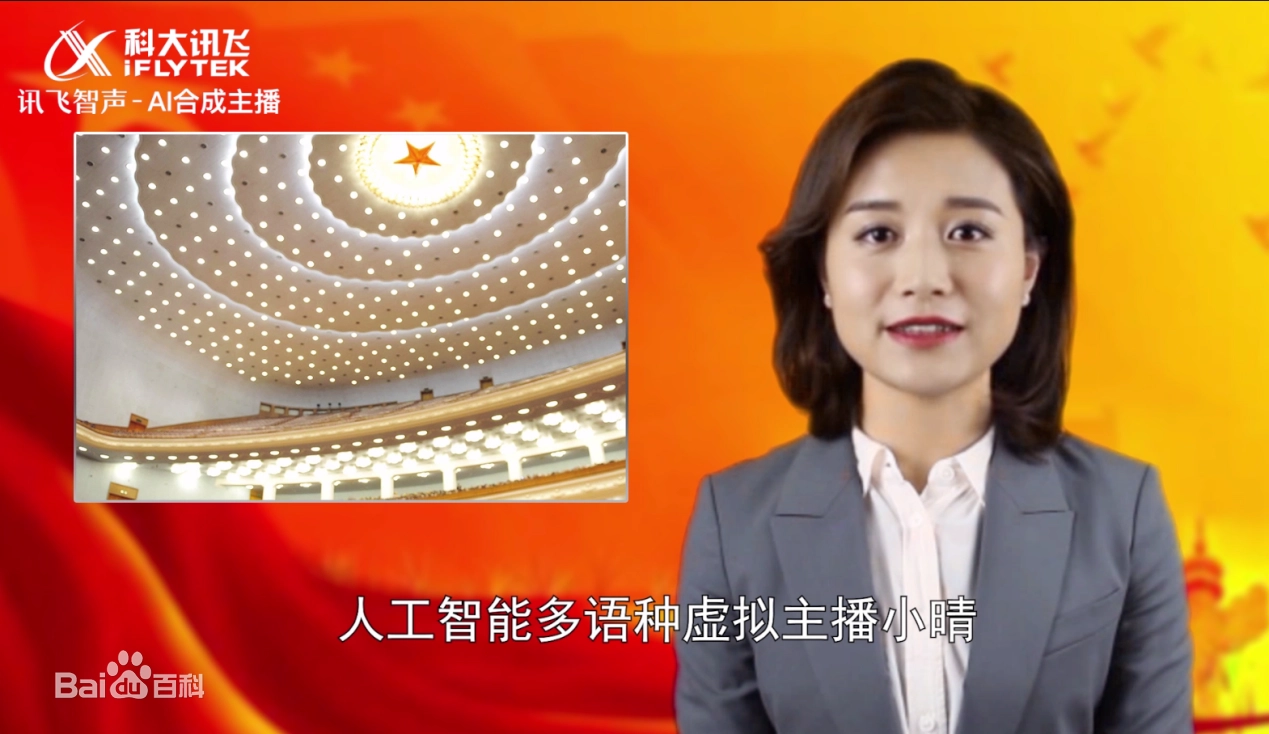
\includegraphics[scale=0.3]{ai主播.png}
    \caption{ai主播}
    \label{fig:example1}
\end{figure}
\section[发展历史]{发展历史\protect\footnote{内容来源:https://baijiahao.baidu.com/s?id=1634743828201865382\&wfr=spider\&for=pc}}
\subsection{1.0时代——雏形初显,虚拟主持人登场}
2001年,世界上第一个虚拟主持人阿娜诺娃(Ananova)诞生了。当时,随着网站经济垮台,互联网泡沫破裂,全球动荡不断。而动荡,对于传媒业来说,往往意味着“富矿”。如何加快新闻生产速度,提升新闻播报的准确率,成为了各家媒体竞争的焦点。英国PA New Media公司正是抓住了这一契机,顺势推出了阿娜诺娃,并将其作为英国传媒业与美联社对抗的“秘密武器”。彼时的阿娜诺娃,虽是一个只有头部动画、表情也略显僵硬的2D虚拟人物,但因可根据新闻脚本快速制作视频,并可24小时持续播报的特点,还是在全球刮起了一阵打造“虚拟主持人”的飓风,如日本推出了寺井有纪(Yuki),中国推出了歌手虚拟主持人阿拉娜(Alana),美国推出了薇薇安(Vivian),韩国推出了露西雅(Lusia)。

但是此股风潮未持续太久,由于早期技术不成熟、成本过大、语音识别和自然语言处理的准确率较低、制作播报视频速度慢等问题,虚拟主持人市场瞬间熄火,并步入了长达十多年的“黑暗时代”。
\subsection{2.0时代——偶像先行,AI虚拟主播顺风飞翔}
2016年,虚拟主播绊爱(kizunaai)在YouTube上首次亮相,虽然其本质为真人扮演,在专业公司制定好绊爱的3D模型后,由真人穿上动捕设备,在背后控制绊爱的面部动态表情及动作,并由声优去配音及对口型,从而进行直播或录制视频,但是从播报状态上来看,无论是3D形象,还是语音、动作,绊爱相比早期主持人都明显更胜一筹。这种整体播报质感和体验的升级,让绊爱几乎在没有任何市场运作的前提下,YouTube订阅数一路扶摇直上,截止目前已超过259万人,从虚拟主播摇身一变为全民偶像。

此外,2016年,AlphaGo以1:4打败围棋世界冠军李世石的事实,让人们意识到,已经诞生了几十年的人工智能,处在了可全面商业化的临界点,AI时代正加速到来。同年,科大讯飞、搜狗、百度先后召开发布会,对外公布语音识别准确率均达到97\%。科技自媒体人阑夕曾说,一旦语音识别的准确率达到99\%,那将直接进入产业爆发的黎明。巧合的是,这一轮AI虚拟主播热潮的兴起,与AI,特别是语音识别技术的飞跃,几乎是同步的。

智能语音产业的发展速度,在某种程度上影响了AI虚拟主播市场化的进度。但在AI虚拟主播的赛道上,虚拟形象的生成与打造,也是一道绕不过去的坎。毕竟,只有声、没有形的主播,只能存在于广播之中。

2018年5月,科大讯飞携手相芯科技打造了虚拟主持人“康晓辉”。这位虚拟主持人有着与真人相似的外形,不仅与央视记者江凯一同主持了《直播长江》安徽篇,还在现场进行了实时互动。相比绊爱,“康晓辉”的一大亮点就在于其背后的虚拟形象生成技术(PTA),该技术让人们摆脱了3D虚拟形象定制所需的高昂成本,只需普通摄像头和一张自拍,就可实时生成与自己相似且更美观的3D虚拟形象。

且先不论“康晓辉”与真人有多相似,但其背后离不开真人的操作,还是暴露了AI虚拟主播的不足。毕竟,用真人驱动虚拟形象,对于传媒业来说,并非是一个最好的解决方案。但“康晓辉”所揭开的瓦片,如同绊爱所带来的曙光一样,还是为传媒业发展指明了一个方向:虚拟主播AI化,势不可挡。

\subsection{3.0时代——全面AI化,虚拟主播走入千家万户}
目前来看,在自然语言处理领域,市场上已涌现了诸如谷歌、微软、思必驰等众多国内外企业;在语音动画合成技术领域上,也涌现了诸如百度、相芯科技、搜狗等国内企业。未来,随着技术加速升级,全AI化的虚拟主播也将加速到来。且相比传统媒体行业的应用,也许在自媒体上,这一愿景将会更早实现。毕竟,从全球市场表现来看,截止2018年底,各大平台上的虚拟主播已经超过了6000个。

AI虚拟主播的实现方式大致可分为三种。一是上述提到的“真人操作”模式,这一模式灵感来源于影视业,实现方式也跟影视业差不多,都需要配套真人演绎,前期需要进行大量的数据采集,中期需要动捕设备来配合播报,后期需要对视频制作进行再加工。从前期准备到后期制作,成本都不可谓不高,这大概也是该模式目前仅限于一些大媒体,难以大范围推广的原因所在。

二是“AR+AI”模式,灵感来源于全息投影,实现方式依赖于增强现实技术。这一模式,需要提前设置好AI虚拟主播的回答、动作、表情等,并通过其与真人主播的互动,来制造真实感。且因为AI虚拟主播是后期做上去的,所以现场真人主持与其互动时,就需要靠“演”。但这种实现方式,对真人主持的要求极高,对后期制作的要求也很高,从应用层面来看,要大范围推广难度显而易见。

三是全AI化模式,灵感来源于早期主持人,实现方式和效果却比早期主持人好很多。这一模式分成定制AI虚拟主播和使用视频制作后台两步,其将上述两种方式中“人”的成分大大剔除,专注于用AI来替代人力,将虚拟主播的语音、情绪、动作,乃至后期视频制作需要的图片、视频等都集成到后台编辑系统中。目前来看,它是更接近全自动化,也更节省制作成本、提升制作效率的方式。相比前两者已有多个应用,全AI化的模式目前落地的项目似乎只有世园会期间,北京电视台和相芯科技联手制作的AI虚拟主播小萌芽、小萌花的播报视频。不过,该视频中的AI虚拟主播,虽然语音、动作、表情等都已接近真人,但形象上仍是3D卡通人物。

迈克斯·泰格在《生命LIFE 3.0》一书中说,生命3.0是一个由人工智能重塑的时代。在这个时代,我们可以设计自己的硬件和软件。这与AI虚拟主播时代,可谓不谋而合。
\chapter{AI主播出现的背景}

\section{AI主播与人工智能技术}
随着人工智能技术的进步,AI主播也在不断发展:

\begin{enumerate}
    \item 自然语言处理(NLP)的进步:NLP技术的发展使得AI主播能够更准确地理解、分析和生成人类语言,包括对话、新闻报道、评论等内容。这使得AI主播能够更加流畅地进行对话,并生成更加自然、符合语境的语言内容。
    \item 语音合成技术的提升:语音合成技术的进步使得AI主播能够生成更加逼真、自然的人类语音,包括语调、语速、音色等方面的模仿。这使得AI主播的表现更加接近人类主播的声音特征,提高了用户的沉浸感和体验质量。
    \item 计算能力的提升:随着计算能力的不断提升,特别是图形处理单元(GPU)和神经网络加速器的应用,使得训练和部署复杂的AI模型变得更加高效和快速。这为开发能够实时处理大量数据并生成复杂表现的AI主播提供了基础条件。
    \item 数据集和算法的丰富:随着大数据时代的到来,人工智能技术所需的数据集和算法得以不断丰富和完善。这为AI主播提供了更多真实场景下的数据支持,使得AI主播在语言表达、情感模拟等方面能够更准确地模仿和表达人类行为。
    \item 多模态技术的应用:人工智能技术的发展使得多模态技术得以应用于AI主播中,包括语音、图像、视频等多种形式的信息处理。这使得AI主播能够在声音、外貌和行为上更全面地模拟人类主播,提高了其在媒体和娱乐产业中的应用价值和实用性。
\end{enumerate}

总体而言,人工智能技术的快速发展为AI主播的出现和发展提供了技术基础和支持。随着技术的不断创新和突破,AI主播在媒体和娱乐产业中的应用前景将会更加广阔,并将不断为用户带来全新的观看和体验方式。
\section{AI主播与个人虚拟社交需求}
个人虚拟社交需求的发展是指个人在虚拟社交平台上与他人进行交流、互动和沟通的需求,这种需求的不断增长推动了AI主播的发展,主要体现在以下几个方面:
\begin{enumerate}
    \item 娱乐需求的增长:随着社交媒体和虚拟社交平台的普及,人们对于娱乐内容的需求不断增长。AI主播作为一种娱乐形式,能够提供更多样化、个性化的娱乐内容,满足用户对于创新、新鲜、有趣内容的追求。
    \item 社交互动的追求:个人在虚拟社交平台上寻求与他人进行交流、互动和分享。AI主播作为虚拟社交平台上的一种内容提供者,能够模拟人类主播的行为和语言,与用户进行交流互动,满足用户在虚拟社交空间中的社交需求。
    \item 个性化体验的要求:随着人们对于个性化体验的追求,AI主播能够根据用户的兴趣爱好、需求偏好等个性化因素,提供符合用户口味的内容推荐和服务。通过分析用户行为和偏好,AI主播能够实现更加精准的内容定制,从而提高用户的满意度和粘性。
    \item 跨时空互动的需求:个人在虚拟社交平台上寻求跨时空的互动和交流,与不同地区、国家的人进行交流和分享。AI主播作为虚拟形象,不受时间和空间限制,能够为用户提供跨地域、跨时区的互动体验,促进人与人之间的跨界沟通和交流。
    \item 虚拟社交的新形式:随着技术的发展,虚拟社交形式不断丰富和创新,AI主播作为其中的一种新型社交形式,为用户带来了全新的社交体验和互动方式。AI主播的发展促进了虚拟社交的多样化和丰富化,拓展了人们在虚拟社交空间中的交流方式和方式。
\end{enumerate}
\section{AI主播与数字化媒体}
数字化媒体是指传统媒体内容、媒体形式和媒体传播过程经过数字化技术加工处理后所呈现的媒体形态。这包括数字化的音频、视频、文字、图像等多种形式的媒体内容,以及通过互联网、移动通信网络等数字化渠道进行传播和交流的媒体形式。数字化媒体的出现和发展,使得媒体内容的生产、传播和消费更加便捷、快捷和个性化,极大地改变了传统媒体产业的格局和模式。
数字化媒体与AI主播发展联系:
\begin{enumerate}
    \item 内容生产与分发:数字化媒体为AI主播提供了更广阔的内容生产和分发平台。AI主播利用数字化媒体平台,可以生产和发布更丰富、多样化的内容形式,包括文字、音频、视频等形式的媒体内容,满足用户对于多样化媒体内容的需求。
    \item 个性化定制服务:数字化媒体平台为AI主播提供了个性化定制服务的实现途径。通过数字化媒体平台的数据分析和个性化推荐技术,AI主播能够更好地了解用户需求和偏好,为用户提供更精准、个性化的内容服务,提高用户体验和满意度。
    \item 用户参与和互动:数字化媒体平台为AI主播与用户之间的互动和参与提供了更广泛的空间。AI主播可以通过数字化媒体平台与用户进行实时互动、社交分享、内容反馈等形式,增强用户与AI主播之间的互动体验和沟通交流,提高用户对于数字化媒体平台的粘性和参与度。
    \item 多媒体形式的创新:数字化媒体为AI主播提供了更多样化、创新性的多媒体形式的创作和表现空间。AI主播可以利用数字化媒体平台的多媒体功能,结合文字、音频、视频等多种形式的内容表现手段,为用户呈现更加丰富、立体化的媒体内容体验,提高内容的吸引力和表现力。
\end{enumerate}
\end{document}